\chapter{Grundlagen}
\section{Distanzmessung mit Ultraschall}
Die Distanzmessung mit Ultraschall ist ein berührungsloses Verfahren. Die Messung erfolgt beruht auf Laufzeitmessung. Der Frequenzbereich von Ultraschalls liegt zwischen 20Khz - 1Ghz (vgl. \cite{ultraschallbereich}) und somit außerhalb des hörbaren Bereichs (20Khz ). \\
Ein Ultraschallsensor besteht aus einer Sende- und Empfangseinheit. Die Schallwellen werden meist auf Basis des piezoelektrischen Effekts impulsartig ausgesandt und ausgewertet.  Der Ultraschallimpuls pflanzt sich mit Schallgeschwindigkeit im Ausbreitungsmedium fort. Das zu messende Objekt reflektiert die Schallwelle. Die Emfpangseinheit nimmt das entstandene Echo auf. Durch die verstrichene Zeit von der Aussendung bis zum Empfangen des Impulses kann die Entfernung des Objektes bestimmt werden. \\

Dabei gilt:
\begin{align}
d = \frac{1}{2} \cdot t\cdot c \\
c \approx 340m/s 
\end{align}

Die maximale Messdistanz hängt dabei von der maximal möglichen Intensität der ausgesandter Wellen ab. Die minimale Messdistanz wird durch die Frequenz der Messung bestimmt. \\
Prinipbedingt unterliegen Ultraschallsensoren einigen Messfehlern. Dazu gehört, dass schallschluckende Oberflächen eine zu geringe Intensität reflektieren. Dasselbe gilt für Objekte mit rauer Oberfläche. Messfehler können außerdem durch sog. Scheinechos entstehen, wenn der Ultraschallimpuls von mehreren Objekten reflektiert wird. Aufgrund des Öffnungswinkels der Schalwelle ist der gleichzeitige Betrieb mehrerer Sensoren nur eingeschränkt möglich. (vgl. \cite{ultraschallUni}; \cite{ultraschallBa})

\section{MQTT} %Acronym wieder einfuegen!
\acrshort{mqtt} ist ein Protokoll, welches zur digitalen Datenübertragung in ethernet-basierten Systemen dient. Es benötigt nur wenig Bandbreite und Ressourcen und verwendet eine 
Publish/Subscribe - Architektur. Das bedeutet, dass Nachrichten sogenannter Topics von Publishern bereitgestellt und von Subscribern empfangen werden. Der Datenverkehr wird über einen 
zentralen Broker verwaltet. Um die Publish Subscribe Architektur zu verstehen ist es hilfreich die Analogie zum Fernsehen zu bilden. Dabei sendet ein TV-Sender sein Programm an einen bestimmten Kanal.
Auf diesen Kanal können nun beliebig viele Fernseher (Subscriber) zugreifen. Auch wenn keine aktive Verbindung zwischen Sender und Empfänger aufgebaut wird, erhalten beliebig viele Empfänger die benötigten Daten.
In \autoref{pic:mqttbroker} ist zu erkennen, wie die Daten nicht zwischen Publisher und Subscriber direkt, sondern über den zentralen Broker versendet werden. (Vgl. \cite{mqtt})

\begin{figure}[h]
    \begin{center}
        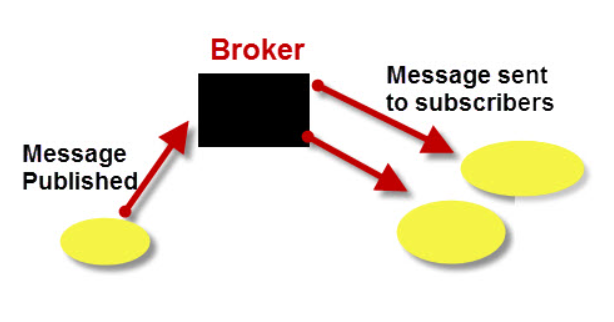
\includegraphics[width=8cm]{mqttbroker.png}
        \caption{\acrshort{mqtt}-Datenübertragung über den Broker}
        \label{pic:mqttbroker}
    \end{center}
\end{figure}